\chapter{Implementation}
\label{sec:implementation}
\index{CRAVA!implementation}

Whereas the general model was explained in \autoref{sec:theory} we
explain a bit more of the actual implementation details here.

The estimation routines implemented in \crava are based on
straightforward and commonly used techniques. This gives fast and
robust estimation, although we may run into problems if the number of
data points is too small, or the data quality is too low. The quality
of an estimation result is never better than the quality of the data
it is based on.

\section{Estimating optimal well location}
The positioning uncertainty between well data and seismic data is
often significant. To overcome this, the well may be moved to the
location with maximum correlation between the seismic data and the
reflection coefficients calculated from the well data. The relation
between the seismic data and reflection coefficients is linear; so
linear covariance is a good measure. The optimal well location is
found by searching for the location with highest covariance in a
lateral neighbourhood around the original well location, where the well
is allowed to be shifted vertically in each target position. The
moving of wells is triggered by a command in the model file, and it is
done prior to the estimation of wavelets, noise, correlations and
background model.

\section{Estimating the prior model}

The prior model for the Bayesian inversion is defined in
equation~\eqref{mdist}, and consists of the expectations of the
elastic parameters $V_p$, $V_s$, and $\rho$ collected in the vector
$\bmu_m$, and their spatial correlation structure collected in the
covariance matrix $\bSigma_m$. These expectations and covariances must
be given prior values before the inversion.

\subsection{Background model}
\index{prior model!background}
\label{sec:backgroundmodel}

The expectation $\bmu_m$ is usually referred to as the background
model. As the seismic data do not contain information about low
frequencies, a background model is built to set the appropriate
levels for the elastic parameters in the inversion volume. To
identify this level, we can plot the frequency content of the seismic
traces in the available wells, and identify lowest frequency for which
seismic data contains enough energy to carry information.

\begin{figure}
\centering
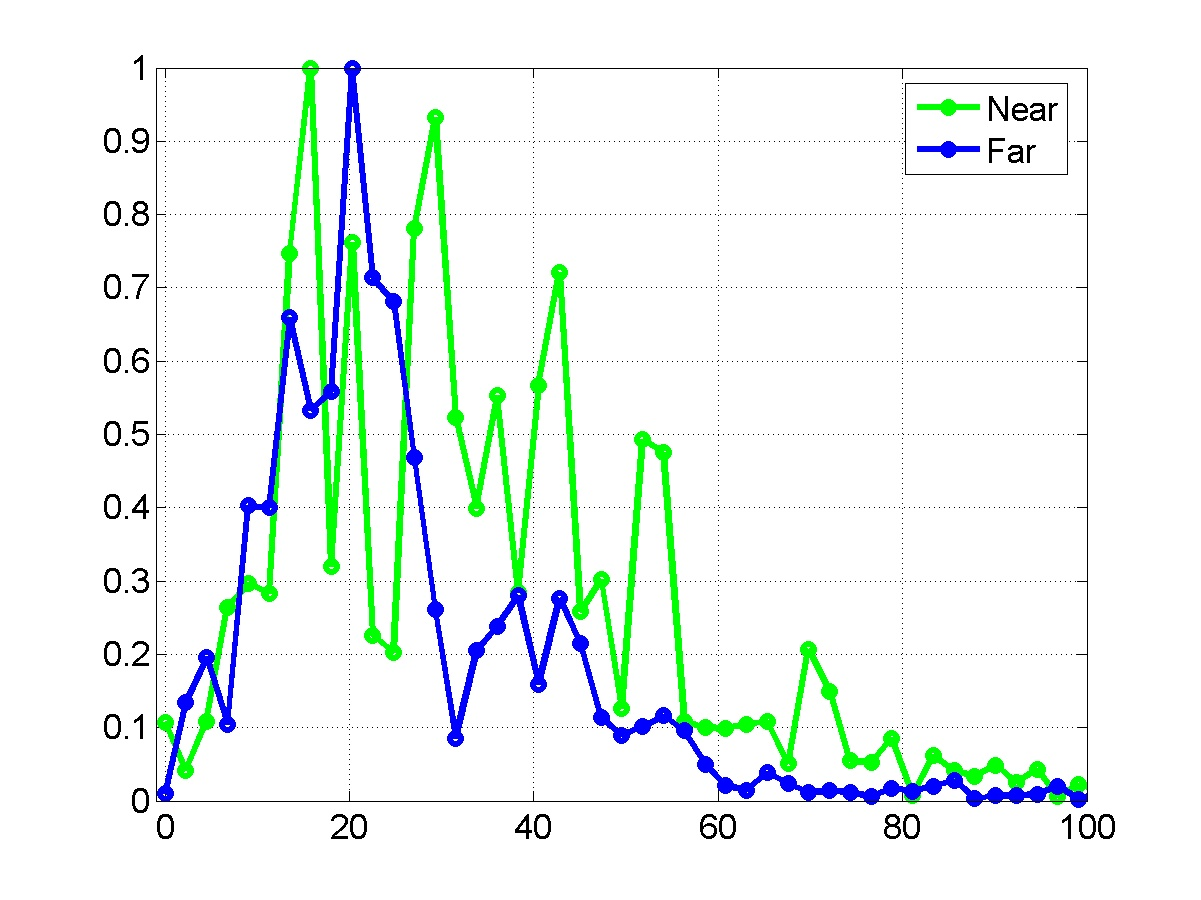
\includegraphics[width=.49\linewidth]{images/implementation/seismicFrequencies_S1}
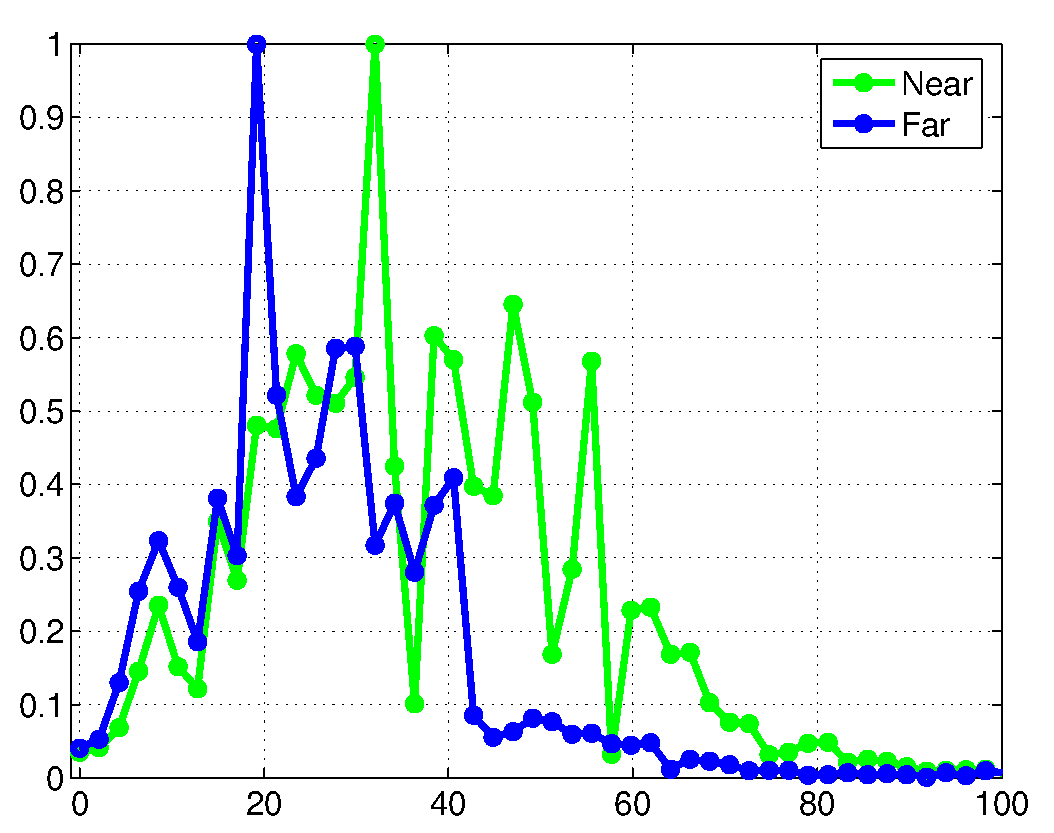
\includegraphics[width=.49\linewidth]{images/implementation/seismicFrequencies_S2}
\caption{The frequency content of the seismic traces in two different
         wells. The frequency content of the near and far stacks are
         shown as green and blue curves respectively.}
\label{fig:frequencycontent}
\end{figure}

In \autoref{fig:frequencycontent}, we have plotted the frequency content
in the seismic data in two different wells. The green curve gives the
frequency content in the near stack and the blue curve gives the
frequency content in the far stack. These plots show that the seismic
data contain little energy below 5--6Hz, and the purpose of the
background model is to fill this void.

The estimation of the background model is made in two steps. First,
we estimate a depth trend for the entire volume, and then we
interpolate well logs into this volume using kriging. The estimation
will by default contain information up to 6Hz, but this high-cut limit
can be adjusted using the \texttt{<high-cut-background-modelling>}
keyword.

When identifying the depth trend, it is important that the wells are
appropriately aligned. The alignment is defined by the time interval
surfaces specified as input, or alternatively, the correlation
direction surface. It is important that the alignment reflects the
correlation structure (deposition/compaction), and if the time
surfaces are either eroding or on-lapped, one should consider specifying
the correlation direction separately using the
\texttt{<correlation-direction>} keyword.

In \autoref{fig:log-aligning}, we show two well logs aligned according
to deposition and according to the true time scale. Evidently, an
incorrect trend will be identified if the true vertical depth is
used. The size of the error will depend on the stratigraphy.

\begin{figure}
\centering
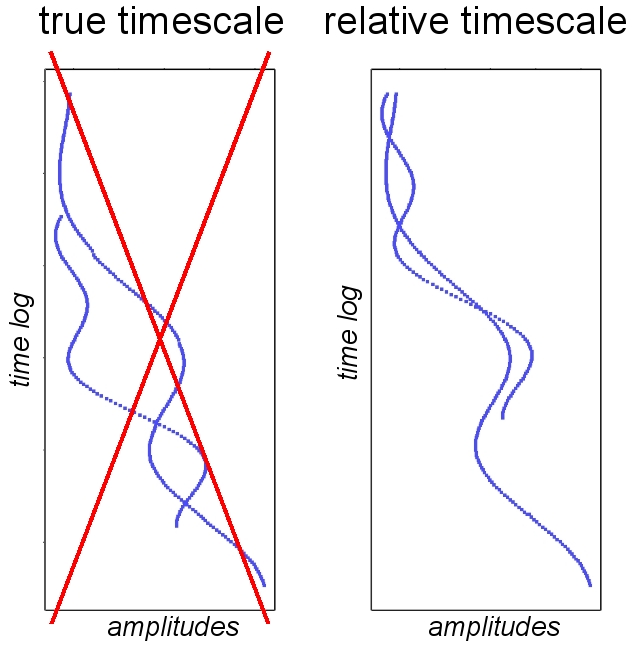
\includegraphics[width=.45\linewidth]{images/implementation/Trend-analysis_dep-vs-comp}
\caption{Well logs aligned according to true time scale (left) and
         according to stratigraphic depth (right).}
\label{fig:log-aligning}
\end{figure}

Assuming properly aligned wells, the trend extraction starts by
calculating an average log value for each layer. This average is
calculated for the \vp, \vs, and $\rho$ well logs and is based on all
available wells. The estimation uses a piecewise linear regression,
rather than the more straightforward arithmetic mean or moving
average, as these measures are sensitive to the amount of data
available. The piecewise regression has the additional advantage
that it can give trend estimates also outside the interval for which
we have data available.

For the linear regression we require a minimum of 10 data points
behind each estimate. In addition, we require that the minimum number
of data points must also be at least 5*N$_\text{wells}$. This way we
ensure that data points from different time samples are always
included. Alternatively, the regression would reduce to an arithmetic
mean whenever there are 10 or more wells available. If we enter a region
with no data points available at all, the minimum requirements are
doubled.

To get the right frequency content in the depth trends, the regression
values are eventually frequency filtered to 6Hz.

The trend extraction process is illustrated in
\autoref{fig:vertical-trends} for the \vp and $\rho$ logs of a field
with six wells. Note that the plots are oriented with layers
as abscissa and log values as ordinate. The blue circles represent log
values from any wells, the green curve is the piecewise linear
regression of these values, and the red curve is the
frequency filtered log that will be used as a depth trend. Note that
the green curve is slightly erratic, especially, as we enter the
region (below reservoir) where there are no data points
available. This shift, which is clearly observed for the density,
arises as we stabilise the estimate by requiring twice as many data
points behind each estimate.

\renewcommand{\floatpagefraction}{0.60}

\begin{figure}
\centering
\fbox{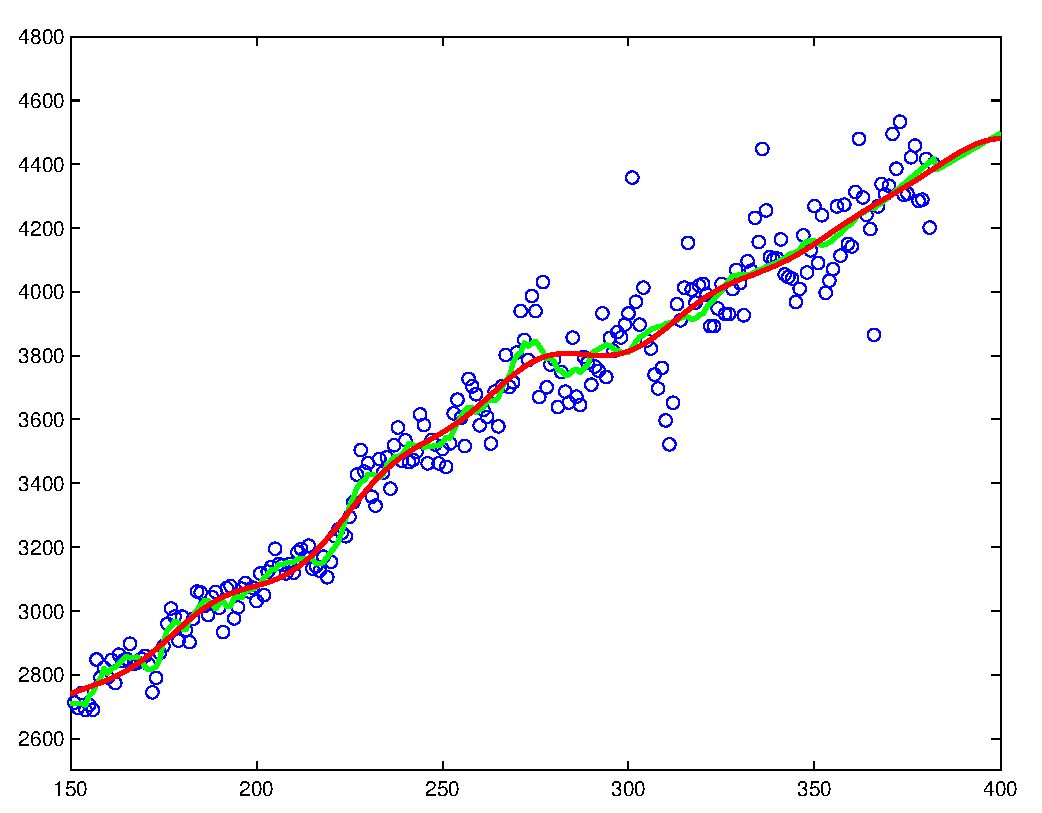
\includegraphics[width=.480\linewidth]{images/implementation/vertical-trend-vp}}
\fbox{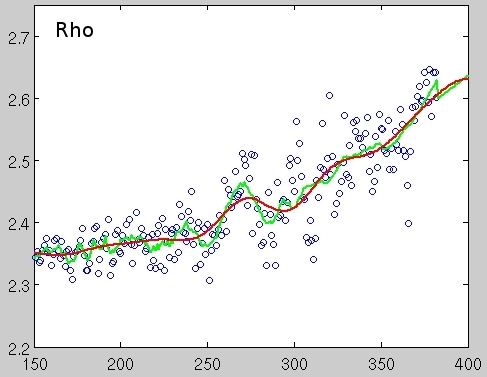
\includegraphics[width=.472\linewidth]{images/implementation/vertical-trend-rho}}
\caption{Well log values plotted against grid layer number for \vp
         (left) and $\rho$ (right). The blue circles show log values,
         the green curve is a piecewise linear regression of the these
         values, and the red curve is the regression values filtered to 6Hz.}
\label{fig:vertical-trends}
%%\end{figure}
%%\begin{figure}
\vspace{1em}
\centering
\fbox{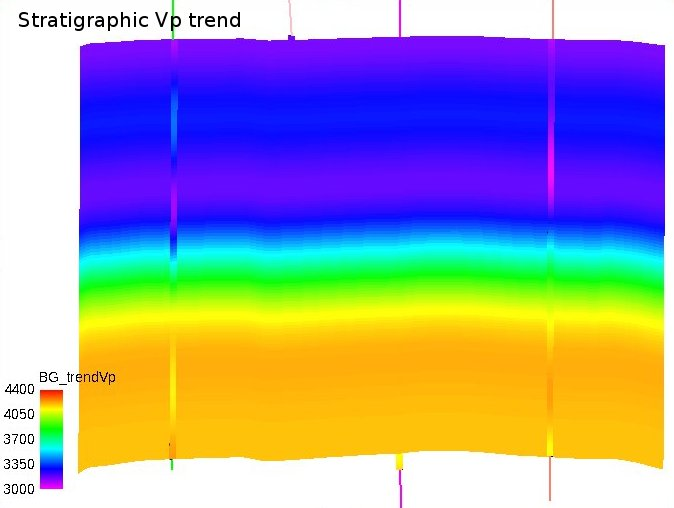
\includegraphics[width=.480\linewidth]{images/implementation/BGtrend_stratigraphic_trend_Vp}}
\fbox{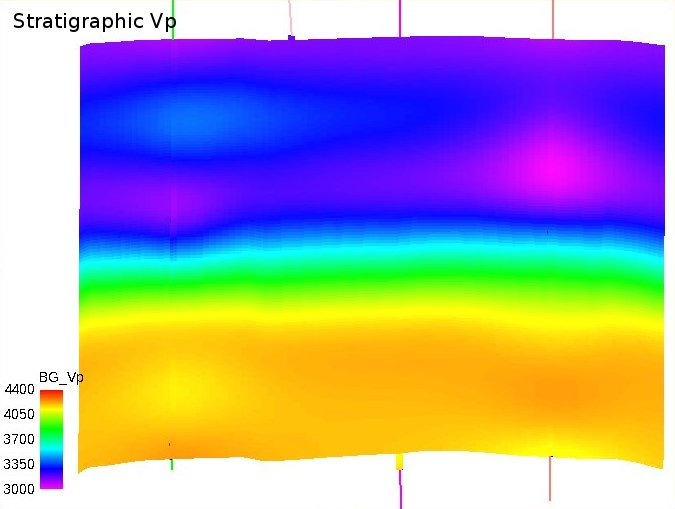
\includegraphics[width=.480\linewidth]{images/implementation/BG_stratigraphic_trend_Vp}}
\caption{\vp depth trend (left) and final background model
  (right). Well logs of \vp, high-cut filtered to 6Hz, are shown for
  comparison.}
\label{fig:background}
\end{figure}

When the inversion volume has been filled with the depth trend, we
interpolate it with 6Hz filtered well logs, to ensure that the
background model will match in wells. A cross section of the resulting
background model for \vp is illustrated in the right part of
\autoref{fig:background}. To the left is the corresponding depth
trend. For comparison the well logs of \vp has plotted in both
illustrations. Note how the wells influence the volume in a region
around the well.

Ideally, the background model should be as smooth as possible,
and a Gaussian variogram model with relatively long ranges may seem an
obvious choice. This model is too smooth, however, and should be
omitted as it often give parameter over- and undershooting away
from wells.

\subsubsection{Multizone background model}
In the \kw{multizone-model}, the reservoir is divided into several horizontal zones defined by surfaces in the inversion volume. In each zone, a local backround model is made by estimating a depth trend for the zone volume, then kriging well logs to the depth trend. The full multizone background model is made from the zone background models by using Beta distributions with $\alpha = \beta =2$ for the transitions between the zones. The limits of the Beta distribution may be different for each surface, and they are given as input to the model. The background model in each zone contains frequencies up to 6Hz, but the frequency content is higher in the transitions between the zones. These higher frequencies will, however, contain information about the locations of the zones; hence they contain important prior information. Higher uncertainty gives smoother background models with lower frequency.

\subsection{Covariance}
\label{sec:correstimp}

Since we model the covariance structure as separable, we have
collapsed the full time dependent covariances between parameters into
one parameter covariance matrix $\bSigma_{0,m}$, a lateral correlation
vector $\cml(\xi)$, and a temporal correlation vector
$\cmt(\tau)$.

We estimate the correlations by first blocking the wells into the
grid, and then do standard correlation estimation using
\begin{equation}
%%\text{Cov}(X,Y) = \text{E}(XY)-E(X)E(Y),\quad\text{with}\quad
%%X,Y\in\{\ln\vp, \ln\vs, \ln\rho\}
\text{Cov}(X,Y) = \frac{\sum(x_i - \bar{x})(y_j - \bar{y})}{\sqrt{n - 1}},\
  \text{with}\ X,Y\in\{\ln\vp, \ln\vs, \ln\rho\}
\end{equation}

The parameter covariance matrix is simply estimated by using the
covariances at time lag 0. In \autoref{fig:parameter-correlation}, we
show cross plots of the parameter residuals ($x_i - \bar{x}$) for a
sample field. The depicted distributions look similar to bivariate
normal distributions, which supports the normal distribution
assumptions made in \autoref{mdist}. If there are no \vs logs
available, the prior \vs variance will be set equal to twice the \vp
variance, and their covariance will be set equal to zero.

The temporal correlation is estimated from the remaining lags in the
well logs as depicted in \autoref{fig:temporal-correlation}. The
temporal correlation will be a weighted average of the estimates made
for all three elastic parameters.

While the covariance matrix and the temporal correlation can be readily
estimated from well data, this is not the case for the lateral
correlation, unless there are a large number of wells available. The
lateral correlation is therefore normally chosen parametric. There is
an option in \crava to estimate the lateral correlation from seismic
data, but these estimates are not made relative to stratigraphy and
tend to grossly underestimate the correlation. Using a parametric
correlation function is therefore encouraged. In
\autoref{fig:lateral-correlation}, we have depicted an exponential
correlation function and the lateral correlation structure this kind
of function gives rise to.

\begin{figure}
  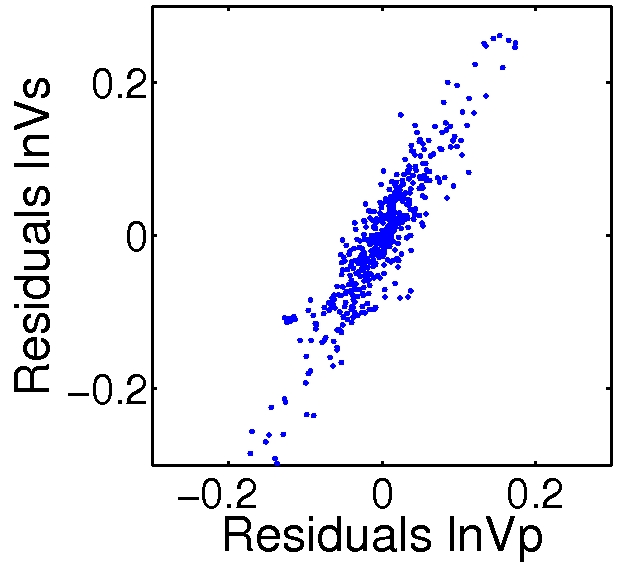
\includegraphics[width=.33\linewidth]{images/implementation/correlation-scatterplot_vp_vs.jpg}
  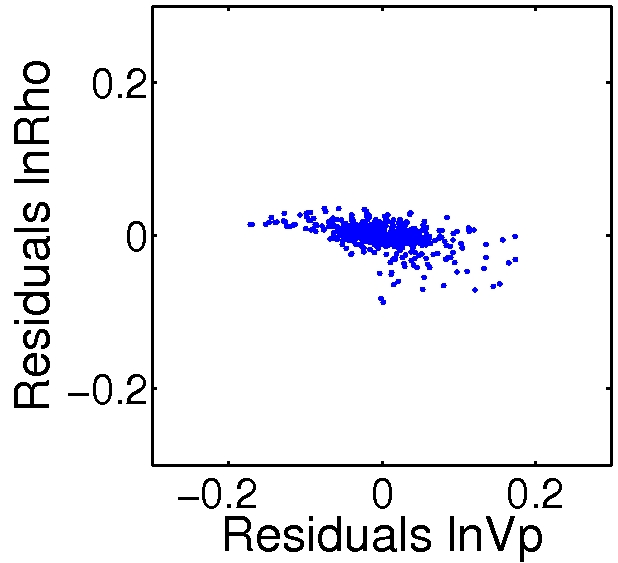
\includegraphics[width=.33\linewidth]{images/implementation/correlation-scatterplot_vp_rho.jpg}
  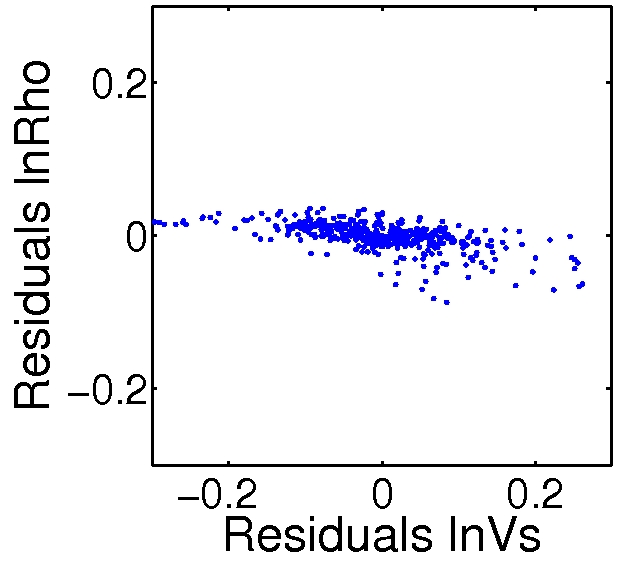
\includegraphics[width=.33\linewidth]{images/implementation/correlation-scatterplot_vs_rho.jpg}
  \caption{Cross plots of logarithmic parameter residuals. From such
           plots the parameter correlations may be estimated.}
  \label{fig:parameter-correlation}
  \vspace{2em}
  \centering
  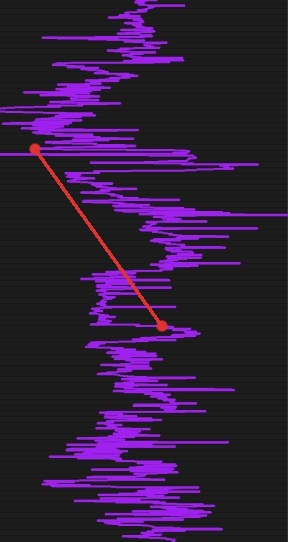
\includegraphics[width=.2\linewidth, height=8.0cm]{images/implementation/temporal_covariance.jpg}\qquad
  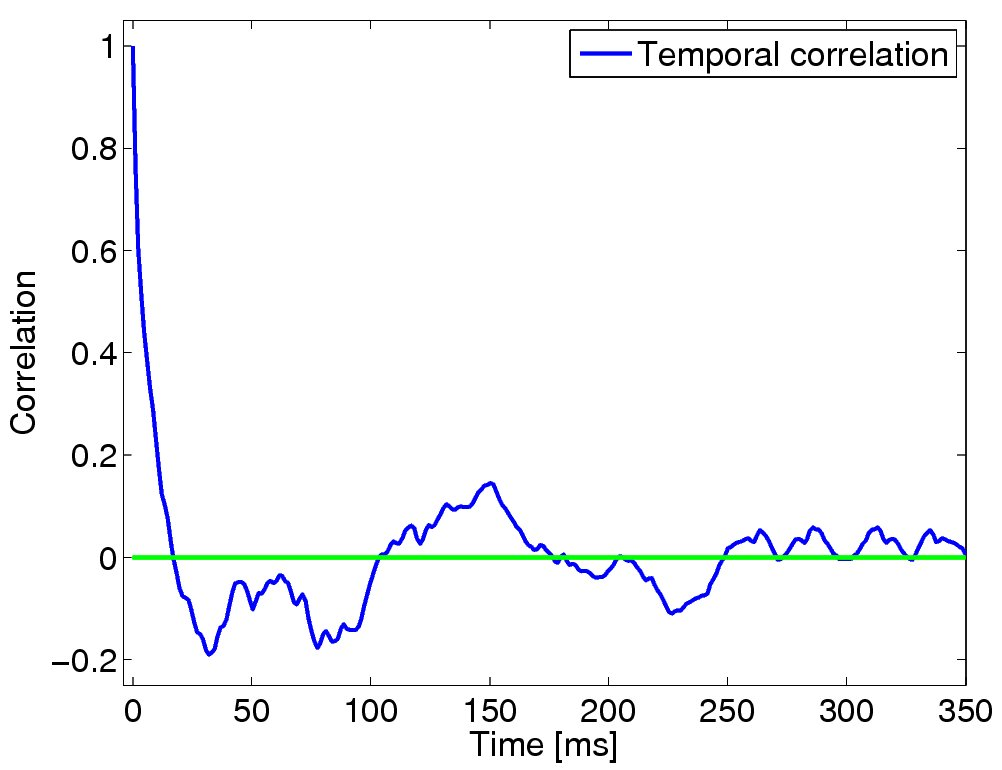
\includegraphics[width=.7\linewidth              ]{images/implementation/temporal_correlation.jpg}
  \caption{We obtain the temporal covariance by measuring the
    covariance between all pairs of points in the well log (left). The
    resulting temporal correlation function (right).}
  \label{fig:temporal-correlation}
  \vspace{2em}
  \centering
  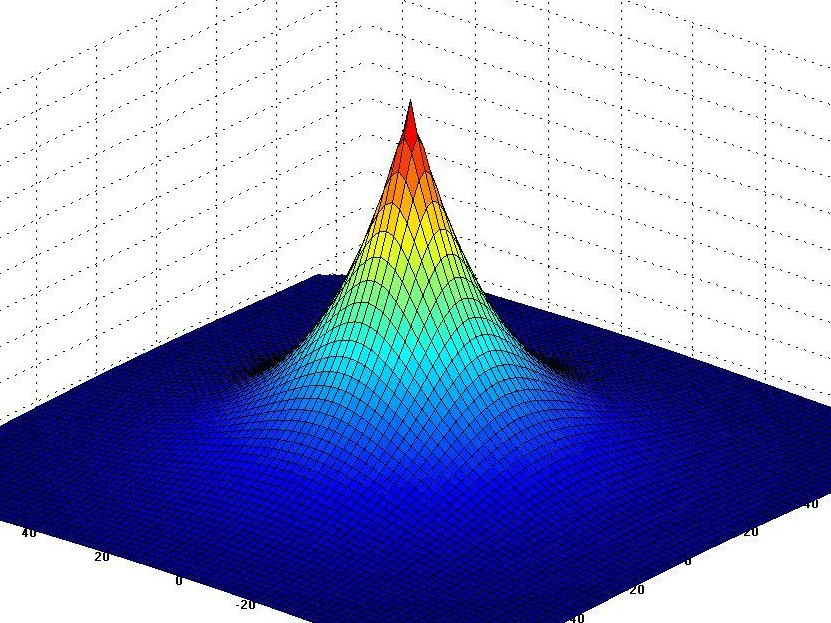
\includegraphics[width=.52\linewidth,height=6cm]{images/implementation/lateral_correlation_1.jpg}\qquad
  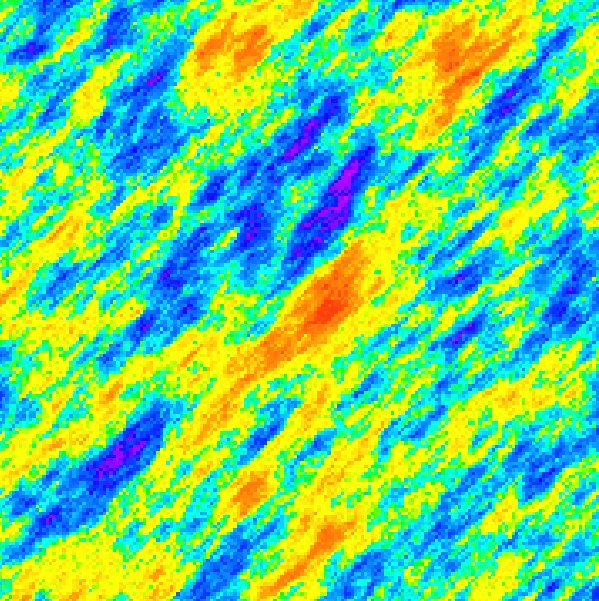
\includegraphics[width=.42\linewidth           ]{images/implementation/lateral_correlation_2.jpg}
  \caption{Parametric lateral correlations. A two-dimensional
    exponential correlation function (left). The lateral correlation
    structure resulting from an anisotropic exponential correlation
    function having an azimuth of $45^\circ$ degrees (right).}
  \label{fig:lateral-correlation}
\end{figure}



\subsection{Likelihood model}

As with the prior model for the elastic parameters, we have also
collapsed the full time dependent error covariance matrix into a noise
covariance matrix $\bSigma_{0,e}$, a lateral correlation vector
$\cel(\xi)$, and a temporal correlation vector $\cet(\tau)$.

The lateral correlation is difficult to estimate and is chosen equal
to that for the elastic parameters, that is, we use $\cel(\xi) =
\cml(\xi)$. The temporal correlation is partly estimated from wavelet
derivatives and partly white noise. By default, a 10\% white noise
fraction is assumed.

For the noise covariance matrix, the noise for a single angle gather
can be either specified in the model file using the
\texttt{<signal-to-noise>} keyword or it can be estimated. A noise
estimate is found by generating synthetic seismic data (see next
section) using the wavelet optimally shifted in each well, and
subtracting this from the seismic data. The remaining part is assumed
to be noise, and we measure the noise energy from this.

The correlation between the noise in different angle stacks is hard to
estimate and is therefore chosen parametric. Typically, an
exponential correlation functions with a range of 10$^\circ$ is
used. In most cases this implies that the noise in the angle stacks
are treated as independent of each other.

\section{Estimating wavelets}
\label{sec:waveestimp}
The implemented wavelet estimation uses the approach of spectral division, see \cite{White84}. 
In this approach an estimate of the cross-correlation between data  
and reflection coefficients, and an estimate of the auto-correlation of reflection coefficients
are used to estimate the wavelet. The methodology requires that the reflection 
coefficients are known,  thus wavelets are estimated at well locations. 
The cross-correlation between data
and reflection coefficients is found by convolving the data with the reflection coefficients, 
and tapering the result. The auto-correlation of the reflection coefficients 
are found similarly by convolving the reflection coefficients with themselves 
and then applying a taper to the result. The tapering is 
performed in order to avoid spurious correlations at large lags.  

Using the standard convolutional relation for seismic data,
\begin{equation}
\vect{d} = \vect{w}*\vect{c}+\vect{e}, \label{fig:syntseis}
\end{equation}
where $\vect{d}$ is the seismic amplitude data, $\vect{w}$ is the
wavelet, $\vect{c}$ the reflection coefficients, and $\vect{e}$ is the
noise. We see that convolving the data with reflection-coefficients, 
transforming to the  Fourier domain, and take the expectation we get
\begin{equation}
d(\omega)\bar{c}(\omega) = w(\omega)|c(\omega)|^2
\end{equation}
Note that the convolution has disappeared, and the equation can be
solved for each frequency $\omega$. We recognise the left hand side as the 
spectre of the cross-correlation between data
and reflection coefficients. And the left hand side as the wavelet multiplied with 
spectre of the auto-correlation of the reflection coefficients. 
This can be obtained by dividing the spectre of the cross-correlation with the 
spectre of the auto-correlation. 

Tapering of the estimated cross-correlation and auto-correlation is required in order to stabilise the estimate. In Crava a Papoulis taper is used. Tapering is equivalent 
to a local smoothing in the frequency domain, thus the resulting wavelet 
estimate will behave smoothly in Fourier domain. 


We find the optimal vertical shift for each well. The global wavelet
is then found by taking the arithmetic average of the zero-phase
wavelets, weighted by the number of samples used from each well.

When using local wavelets, we find the optimal shift and/or scale of
the global wavelet at each well location. Optimal here means
minimising the noise energy. We then use kriging to interpolate this
between wells, with a shift of 0 and a scale of 1 as the mean level
outside the well control area.  This is illustrated in
\autoref{fig:local-wavelet}.

\begin{figure}
  \centering
  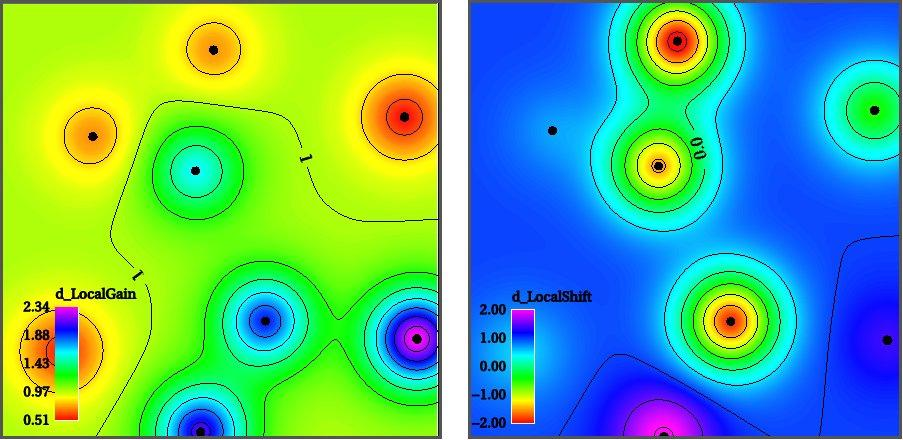
\includegraphics[width=.95\linewidth]{images/local-wavelet}
  \caption{The local scale and shift maps involved when using local wavelets}
  \label{fig:local-wavelet}
\end{figure}

Local noise is estimated using the local noise energies from above. We always use local shift when estimating the noise, but only use local scale if it is used in the inversion. If local scale is used, the noise is divided by this. A noise scaling factor is then computed in each well, and kriged as above.

\section{Estimating 3D wavelet}
\label{sec:3Dwaveestimp}
The expression for the wavenumber representation of the point-spread function given in \autoref{eq:waveletform}
has only one unknown element, namely the 1D pulse $w_0(\omega)$. The functions $\tilde{\alpha}_1$ and $\tilde{H}$ are given as input, together with the average velocity $V_0$. The elements needed for the conversion from depth to time are also input to \crava. That is the reference depth $Z_0$, and reference time surface $T_0$. The theory for the estimation of the 1D pulse is given in \cite{georgsen10}, and with more details in \cite{sand1010}.

As for the 1D wavelet, the pulse is estimated from wells. Using
reflection coefficients from well logs, time gradients estimated from
seismic data around wells and depth gradients computed from time
gradients by using the reference time surface and average velocity given, a matrix $K$ can be constructed forming a linear regression model for the seismic
data as
\begin{equation}
\vect{d} = \vect{K}\vect{w}_0 + \vect{e}.
\end{equation}
The least squares estimate for $\vect{w}_0$ is
\begin{equation}
\widehat{w}_0 = (\vect{K}'\vect{K})^{-1}\vect{G}'\vect{d}.
\end{equation}

\section{Using FFT for inversion}
As previously stated, \autoref{eq:WADm} separates when transformed
into the Fourier domain. After this transformation, the equation
becomes
\begin{equation}
\label{eq:fourierinv}
\vect{\tilde{d}}(\omega,\vect{k}) = \vect{G}(\omega)\vect{\tilde{m}}(\omega,\vect{k}) + \vect{\tilde{e}}(\omega,\vect{k}))
\end{equation}
The tilde denotes the 3D Fourier transform, with temporal
frequency $\omega$, and lateral frequency vector $\vect{k} =
(k_x,k_y)$. Due to the separation, we now have a set of $n$ small
equations, where $n$ is the number of grid cells in the inversion
volume. Everything is still normally distributed, so the solution to
this equation follows the pattern from \autoref{eq:mupost} and
\autoref{eq:sigmapost}. We still must invert a data covariance matrix,
but whereas this matrix had dimension $(n\cdot n_\theta)^2$ before the
Fourier-transform, the matrix we must invert here is reduced to
dimension $n_\theta^2$, where $n_\theta$ is the number of angle
stacks. Since the time for a matrix inversion is almost cubic in size,
it is much faster to invert $n$ of these small matrixes than the one
large. After solving for $\vect{\tilde{m}}(\omega,\vect{k})$, we do
the inverse transform of this to obtain the distribution for
$\vect{m}$. The same does of course hold when we are using local
wavelets that are divided out in advance, \autoref{eq:ADm}. For full
details, see \cite{geo68ab2}.

\section{A note one local wavelet and noise}
\label{sec:nonstationaryimp}
As shown, even though the use of FFT-transform requires stationarity,
we are able to work around this. Wavelets can be made local since
these can be divided out before solving the equations, and locally
higher noise levels can be approximated by interpolating the low-noise
solution and the prior distribution.

\subsection{Local wavelet - dividing out the wavelet}
\label{sec:divwavimp}
A simple division of data by wavelet can easily be done in the Fourier
domain, where the convolution reduces to a multiplication, and the
division can be done one frequency at a time. However, this is very
unstable for frequencies where the wavelet is very weak or not
present, and some sort of stabilisation is needed.

In \crava this is done in two ways. First, we set an upper and lower
cutoff frequency for the wavelet, default set to 5 and 55
Hz. Furthermore, for frequencies that fall below 10\% of the average
amplitude, we set the amplitude to 10\% of average before doing the
division.

\subsection{Local noise}
\label{sec:localnoiseimp}
Local noise is implemented by first finding the solution using the
minimum noise level, to fulfil the stationarity requirements of the
FFT algorithm. We then interpolate the values for each locations
between the prior and this minimum noise posterior. When doing this
interpolation, we ignore correlation between locations. This is not a
problem as long as the noise varies slowly and smoothly.


For each location $\vect{x}$ the adjusted estimate $\tilde{\bmu}_{m|d_{obs}}(\vect{x})$, is found
from the inversion result $\bmu_{m|d_{obs}}(\vect{x})$ by a linear relation,
\begin{equation} \label{eq:LocalAdjustment}
\tilde{\bmu}_{m|d_{obs}}(\vect{x}) = \bmu_{m}(\vect{x}) +\vect{H_x}\left(\bmu_{m|d_{obs}}(\vect{x})-\bmu_{m}(\vect{x})\right),
\end{equation}
The matrix $\vect{H_x}$ is a shrinkage matrix, i.e. the adjusted estimate
is always closer to the prior mean than the inversion result. The matrix
$\vect{H_x}$ depends on the local error variance
 $\bSigma_{e}^x$ and error variance used in the inversion $\bSigma_{e}^0$.

To find the shrinkage matrix we first identify a matrix $\vect{G}_0$
which maps the local prior distribution to the local posterior
distribution when it is observed with the noise $\Sigma_{e}^0$, that is,
$$ \vect{d}(\vect{x}) = \vect{G}_0\vect{m}(\vect{x})+\vect{e}_0,$$
where $\vect{e}_0\sim N\left( \vect{0},\Sigma_{e}^0\right)$.
The inversion of this expression is a linear relation
 \begin{equation} \label{eq:PSigmae}
\bmu_{m|d_{obs}} =\bmu_{m} +\vect{P}(\Sigma_{e}^0)\left(\vect{d}_{obs}-\bmu_{d}\right)
\end{equation}
where  $\vect{P}(\Sigma_{e}^0)=\bSigma_{m}\vect{G}_0^T \left( \vect{G}_0\bSigma_{m}\vect{G_0}^T+\bSigma_{e}^0\right)^{-1}$.

We then define the shrinkage matrix to be:
\begin{equation}\label{eq:H}
\vect{H_x}(\Sigma_{e}^\vect{x},\Sigma_{e}^0) = \vect{P}(\Sigma_{e}^\vect{x})\vect{P}(\Sigma_{e}^0)^{-1}.
\end{equation}
This removes the effect of the standard inversion and add the effect
of the locally adapted inversion. The matrix $\vect{P}(\Sigma_{e}^0)$
is not invertible, but since the local noise always is larger than the
noise in the inversion the product in expression $\ref{eq:H}$ is
always well defined.

\section{Memory handling}
Since the grids needed by \crava can become very large, we try to
keep the number of grids kept simultaneously in memory as small as
possible. This implies that some allocated grids will be used for more
than one purpose. Both padded and unpadded grids are used in \crava,
The amount of memory needed by padded and unpadded grids are
denoted $s_p$ and $s_u$ respectively.
%%The number of padded grids used are counted in detail, while the unpadded grids are
%%only counted in memory computations. In the following, any mention of grid
%%means padded, unpadded will be explicitly stated.

\crava also has an option to use disk space for intermediate storage
of grids. This will reduce the memory consumption with a factor of at
least 2 in realistic cases, but will also increase the computation
time by a factor of almost 3.

\subsection{Grid allocation with all grids in memory}
If intermediate disk storage is not used, the grid memory allocation
will go as follows:

\begin{enumerate}
\item Background grids for Vp, Vs and density, 3 grids.
\item If the background model is to be estimated, another 3 grids are
  allocated for estimation, but destroyed before any other
  allocations.
\item Seismic grids, $n_\theta$. If well optimisation is used, this
  will come before background grids.
\item Possibly prior facies probability grids, indicated by $I_p$,
  $n_f$ unpadded grids.
\item Prior covariance, 6 grids.
\item If relative facies probabilities or local noise, a copy of
  background indicated by $I_b$, 3 grids.
\item {\bf Peak:} At this stage, \crava reaches its first memory
  peak. Minimum memory in use is 10 grids, typical situation with
  three seismic grids and facies modelling requires 15 grids.\\
    Memory usage: $P_1 = (9+n_\theta+I_b*3)*s_p+I_p*n_f*s_u$.
\item The posterior distribution is computed into the background and
  prior covariance grids, and seismic residuals are computed into the
  seismic grids. Thus, the inversion requires no extra grids. (But we
  needed a copy of the background for local noise or facies.)
\item After the inversion, the seismic grids are released, taking us
  off peak down to a base level: \\
  Memory usage:  $P_\text{base} = (9+I_b*3)*s_p+I_p*n_f*s_u$.
\item If simulation is used:
\begin{enumerate}
\item Simulated grids are allocated, 3 grids.
\item If secondary elastic parameters are requested as output (AI,
  $\mu\rho$, etc.), indicated by $I_s$, a computation grid is
  allocated, 1 grid.
\item If kriging is used, indicated by $I_k$, 1 unpadded grid, not
  concurrent with computation grid.
\end{enumerate}
\item {\bf Peak:} New possible peak, since the number of grids now
  allocated may be larger than the released seismic grids. \\
    Memory usage: $P_2 = (12+I_b*3+I_s)*s_p + (I_p*n_f + \max(0,I_k-I_s))*s_u$.
\item New release of grids, back to $P_\text{base}$.
\item If facies probabilities:
\begin{enumerate}
\item 3D histograms of elastic parameters per facies are created, each
  of size 2MB, $n_f$ special grids.
\item Facies probability grids are created, including for undefined,
  $n_f+1$ unpadded grids.
\end{enumerate}
\item {\bf Peak:} New possible peak, since the new memory allocated
  may be larger than the released seismic grids and/or the
  simulation+computation/kriging grids. \\
    Memory usage: $P_3 = (9+I_b*3)*s_p+(I_p*n_f + n_f +1)*s_u + 2*n_f$.
\item Can now release all grids related to facies probability, memory down to $9*s_p$.
\item Eventual kriging of prediction allocates 1 unpadded grid.
\item Everything released.
\end{enumerate}

The maximum memory usage is thus the largest of the actual peaks. The
maximum number of allocated padded grids will occur at either $P_1$ or
$P_2$, whereas the largest number of other grids are allocated at
$P_3$.

\section{Implementation of the rock physics template model}
\label{sec:rf}
The rock physics template model is very flexible, and requires an equally flexible implementation. There are four main elements:
\begin{enumerate}
\item Fluids.
\item Solids.
\item Rocks.
\item Dry-rocks.
\end{enumerate}
We handle these by a dual set of corresponding classes, the distribution classes and the sample classes. We have the set of DistributionFluid, DistributionSolid etc. base classes. These describe the prior distribution for different elements. From these, we can generate samples of the element. These samples are of base classes Fluid, Solid etc., and correspond directly to the Distribution-classes.

Under the base classes, we have a set of derived classes, based on different rock physics models for mixing. These aoos exist on both distribution and sample version. Thus, the tree-like structure of a rock physics template model is mirrored here, with each prior distribution being built as a tree of Distribution... objects, and capable of generating a sample that is a similar tree of sample objects. The sample tree computes it properties as it is built, so the top level knows the resulting elastic parameters.

A feature of the rock physics implementation is that we can update a sample to generate a new sample. This new sample will be highly correlated with the initial sample. This is utilised to generate synthetic well data (for filtering), and when doing 4D modelling. In order to do this updating, each sample stores all the quantiles for the randomly drawn parameters in the sample. When updating a sample, each quantile $u$ is perturbated to a quantile $u_p$ as follows:
\begin{eqnarray}
x = \Phi^{-1}(u) \\
x_p = x + \epsilon \\
u_p = \Phi(x_p).
\end{eqnarray}
Here, $\epsilon$ is normally distributed with expectation 0, and a variance based on the desired correlation. This sampling models the realtion between the existing and new value as a Gaussian pair copula, with a given correlation parameter.

The correlation parameter is controlled in different ways, depending on whether we are generating synthetic wells or setting up a 4D model. In the former case, we use a constant correlation for all random parameters in the sample-tree. This correlation is tuned to obtain the desired correlation between neighbouring samples. In the 4D setting, each random parameter is assigned a yearly correlation (on the distribution level). From this, the correlation for the relevant time step is computed and used for updating. By setting most parameters perfectly correlated, this allows us to update only parameters that are changing in a 4D setting, such as saturation.

\section{Facies probabilities}
How facies probabilities are calculated depends on the input to \crava. If facies probabilities from rock physics is requested, \crava will make synthetic wells from the rock physics models. If rock physics is not used and there are real wells supplied in the input, \crava will make use of these. In both cases, the wells are filtered and used to make a smooth probability distribution from the histogram of observed values. 
\subsection{Trends}
With rock physics, it is also possible to have zero, one or two trends. Trend minimum and maximum values are specified by the user. If the maximum trend value is equal to the minimum value, this is interpreted as having no trend. Each trend axis is divided in 20 bins. Since the grids in general are very large, it is advantageous to keep the number of dimensions low. When there are either one or two trend dimensions, \crava will automatically reduce the three elastic dimensions to the two components that are best resolved by seismic. By minimizing the expression 
\label{eq:geneig}
\begin{equation}
\min_\vect{v} = \frac{\vect{v}^T \vect{\Sigma}_{m|d}\vect{v}}{\vect{v}^T \vect{\Sigma}_{m}\vect{v}}
\end{equation}
once, the best resolved feature is found. The second best feature is found by minimizing the same expression but with the additional constraint of being uncorrelated to the first component. This amounts to choosing the eigenvectors of $\vect{\Sigma}_{m}^{-1}\vect{\Sigma}_{m|d}$ sorted in increasing order of the corresponding eigenvalues. However, the use of trends will increase the number of numerical grids in use in \crava :
\begin{enumerate}
\item With real wells and no rock physics: the wells are filtered and a 3D grid (where the three dimensions represent the three elastic parameters) is filled with the observed values.
\item If facies probabilites from rock physics is requested:
\begin{enumerate}
\item With no trend, a 3D grid is filled with values from the synthetic wells. 
\item With one trend, the three elastic dimensions are reduced to two dimensions and 20 (the number of bins in the trend dimension) 2D grids (actually 3D grids where only two dimensions are in use) are filled.
\item With two trends, the three elastic dimensions are reduced to two dimensions and $20^2=4000$ (the number of bins in the trend dimension) 2D grids (actually 3D grids where only two dimensions are in use) are filled.
\end{enumerate}
\end{enumerate}

\subsection{Synthetic wells}
When rock physics is used, 10 synthetic wells, each of minimum length 100 bins, is simulated per combination of trend parameters. If no trends are used, 10 such wells are simulated. The synthetic wells are made as follows:
\begin{enumerate}
\item If the length of the well is less than 100 bins, draw one of the relevant facies from a uniform distribution (no correlation with the facies above).
\item Draw a facies length from a geometric distribution with expectation 10 ms.
\item Generate a well sample of this length by calling the functionality described in section~\ref{sec:rf} and add this piece to the well.
\end{enumerate}

\subsection{Well filtering and smoothing}
The final probability distribution is smoothed with the seismic uncertainty. This uncertainty is calculated using the prior and posterior spatial covariance for the elastic parameters in the well. For both real and synthetic wells, the distribution of the error in the inversion is calculated as
\label{eq:}
\begin{equation}
\vect{\Sigma}_{e^*,w} = \vect{\Sigma}_{m,w|d} - \vect{\Sigma}_{m,w|d} \vect{\Sigma}_{m,w}^{-1} \vect{\Sigma}_{m,w|d}
\end{equation}
Each well is filtered independently. (...) The bins in the probability grids (one per facies) are then filled with the values from the wells and a Gaussian distribution with covariance in the elastic dimensions from the well filter is created. The facies probability grids are then convoluted with the Gaussian distribution by FFT. This gives $ \hat{p}(\hat{\vect{m}}_i|f_i,\vect{z}) $.
\subsection{Calculating facies probabilities}
The final lithology prediction is computed as
\begin{equation}
\hat{p}(f_i|\hat{m}_i,z) = \frac{\hat{p}(\hat{\vect{m}}_i|f_i,\vect{z}) p(f_i|\vect{z})}{\Sigma_{f_i} \hat{p}(\hat{\vect{m}}_i|f_i,\vect{z}) p(f_i|\vect{z})}
\end{equation} 
The \kw{uncertainty-level} is part of the input to \crava and specifies the likelihood for undefined lithologies. This value is scaled according to the size of the grid, but will result in a high probability for undefined facies if the relevant point is not close to one of the modes in the distribution.